\documentclass{article}
\usepackage{spconf,amsmath,amssymb,graphicx,booktabs}
\graphicspath{{figures/}}
\usepackage{stfloats}
\renewcommand{\topfraction}{0.9}
\renewcommand{\dbltopfraction}{0.9}
\renewcommand{\bottomfraction}{0.9}
\renewcommand{\textfraction}{0.07}
\renewcommand{\floatpagefraction}{0.75}
\renewcommand{\dblfloatpagefraction}{0.75}
\setcounter{topnumber}{3}
\setcounter{dbltopnumber}{3}

\title{GAUSSIAN AVATARS FOR PERSONALIZED SIGN LANGUAGE GENERATION}
\name{Anol Adib Hossain$^{\star}$ \qquad Seungryul Baek$^{\dagger}$ \qquad Kyoojae Shin$^{\star}$
  \thanks{Author order and affiliations to be confirmed before submission.}}
\address{$^{\star}$Dept. of Artificial Intelligence and Electronic Convergence,
  Busan University of Foreign Studies, Republic of Korea \\
  $^{\dagger}$Ulsan National Institute of Science and Technology (UNIST), Republic of Korea}

\begin{document}
\ninept
\topmargin=0mm
\maketitle

\begin{abstract}
We generate sign language video of an arbitrary person from a single photograph
and a text prompt, composing a frozen single-image avatar reconstructor with a
frozen text-to-motion diffusion model in a shared SMPL-X pose space. Measured
against real signing, the motion model reaches 5\% of ground-truth hand
articulation and inverts the natural dominance asymmetry. We correct this two
ways: first, adaptation under a preservation constraint that we show is the
closed-form reduction of a reference-model KL divergence; second, a training-free
per-hand refiner whose affine form provably preserves the mean pose and the
trajectory shape. Together they bring held-out articulation from 0.05 to 1.04 of
real signing while moving a validated sign-correctness score by only $+0.009$.
Because the refiner cannot alter sign identity by construction, we can then
establish what a statistic alone could not: articulation and sign correctness are
independent axes here, and moving one does not move the other.
\end{abstract}

\begin{keywords}
Sign language production, motion generation, diffusion models, cross-lingual
adaptation, generative model evaluation
\end{keywords}



\section{Introduction}
\label{sec:intro}

Sign languages are the primary languages of an estimated 70 million deaf people.
They are not transcriptions of spoken language: they have their own grammar, and
their meaning is carried substantially by the hands. Rendering text as signed
video would make written content accessible in a first language rather than a
second, but signed video needs a signer, and a recorded human does not scale
while a generic avatar discards the personal presence face-to-face languages
depend on. We therefore address the following task: given one photograph of an
arbitrary person and a prompt naming a sign, generate video of that person
performing it, with no per-subject capture, optimization or fine-tuning. The
requirement is a separation of concerns---motion depends only on the prompt,
identity only on the photograph.

Building this today means composing pretrained parts, since paired
photograph-to-sign-video data does not exist at the scale a joint model would
need. Text-to-sign systems have progressed from pose-sequence
regression~\cite{saunders2020progressive} to diffusion over parametric body
representations~\cite{baltatzis2024nsa}, with recent work generating SMPL-X
motion directly~\cite{dong2024signavatar,zuo2025soke} so that output drives 3D
avatars rather than 2D skeletons. Our motion branch~\cite{bensabath2026handmdm}
belongs to this family and is one of very few sign motion models with publicly
released weights, which is why it serves as both the component we adapt and the
baseline we measure against. Most such work targets sentence-level production on
continuous corpora; we work at the level of isolated signs, so there is a single
correct target per prompt and retrieval against real clips of the same gloss is
well posed. For identity, 3D Gaussian splatting~\cite{kerbl20233dgs} has made
single-image animatable reconstruction practical, and we use such a
reconstructor~\cite{qiu2025lhm} frozen. Both branches meet in a shared parametric
pose space, and our contribution sits in the motion path between them.

\noindent\textbf{A measured failure.} Against real signing in the same pose
space, the pretrained motion model reaches 5\% of ground-truth hand articulation,
and it inverts the natural dominance asymmetry of signing. The hands carry the
linguistic content, and the model is quietest exactly where it should be loudest.

\noindent\textbf{A derived preservation objective.} Adapting to a new sign
language from a small corpus requires constraining the model against its
pretrained self, and that constraint is not arbitrary: for a fixed-variance,
$x_0$-parameterized diffusion model, the KL divergence between the adapted and
reference reverse processes reduces exactly to output distillation weighted per
timestep by $w_t = c_t^2/2\sigma_t^2$. The uniform penalty usually written down
is the $w_t \equiv 1$ case, and on our schedule the weighting spans six orders of
magnitude, so we sweep both. Constraining a model against its own initialization
is established elsewhere~\cite{ruiz2023dreambooth,ouyang2022rlhf}, while KL terms
in sign language production serve a different role, regularizing an encoder
posterior against a latent prior~\cite{faure2026vae,higgins2017betavae}; to our
knowledge reference-model preservation has not been applied to adapting a sign
motion generator.

\noindent\textbf{A refiner with invariants.} Rather than balancing articulation
against adaptation inside a loss, we correct it explicitly. Because articulation
as we define it scales quadratically under rescaling of deviations about the
temporal mean, the gain attaining a target follows in closed form, per hand. The
correction is affine about that mean and therefore provably mean-preserving and
shape-preserving: it can restore articulation and cannot reorder or reshape the
trajectory that identifies the sign.

\noindent\textbf{What the invariants buy.} That guarantee makes our main result
readable. Adaptation moves articulation from 5\% to 104\% of real signing, and a
single hyperparameter moves it back to 4\%. Across that range sign correctness
does not change: retrieval stays near chance against a validated 0.498 ceiling,
and the faithfulness diagnostic of~\cite{hong2026collapse} remains at random
alignment under every configuration, including training from scratch, which rules
out cross-lingual transfer as the cause. A correction that damaged the signs
would produce the same flat reading; the invariants exclude that, so the two axes
are demonstrably independent. This bears directly on what the motion statistics
this field reports can be taken to mean---Hong and
Ko\v{s}eck\'{a}~\cite{hong2026collapse} show that FID and BLEU can both improve
while a generator becomes effectively text-independent---so we validate every
metric before it supports a claim: retrieval by leave-one-out on real clips, the
sign spotter by a negative control on its own reference set, and the generator's
run-to-run variability by direct measurement. These checks overturned several of
our own intermediate findings.

\begin{figure*}[t]
  \centering
  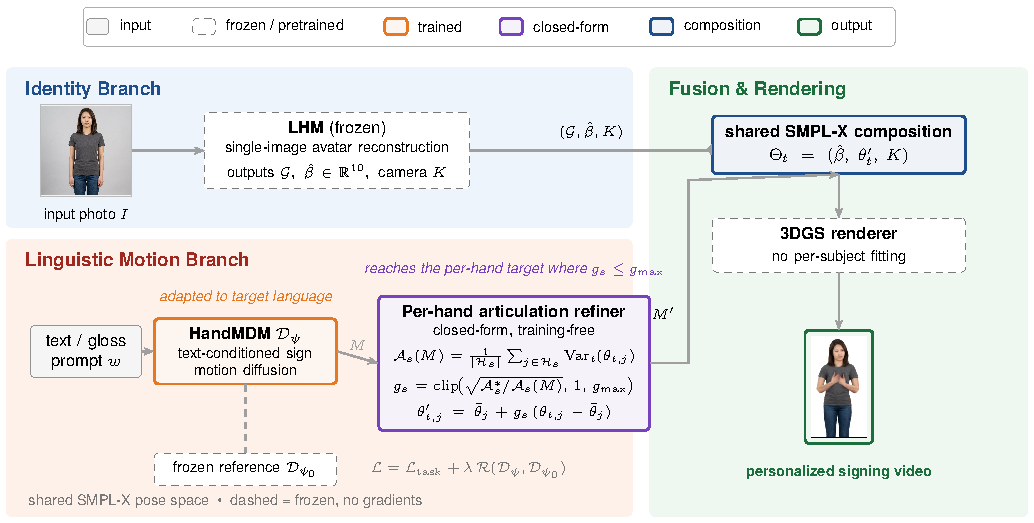
\includegraphics[width=\textwidth]{fig1_pipeline.pdf}
  \caption{Given a reference photograph and a text prompt, a frozen avatar
  reconstructor supplies body shape and camera while a cross-lingually adapted
  motion model supplies the pose sequence. Motion passes through a closed-form
  per-hand articulation refiner, and the two streams are composed in shared
  SMPL-X parameters before rasterisation. Only the motion model is trained,
  constrained against a frozen copy of itself with weight $\lambda$; the refiner
  has no learned parameters and the rendering path requires no per-subject
  optimisation.}
  \label{fig:pipeline}
\end{figure*}

\section{Method}
\label{sec:method}

\subsection{Two-branch composition}
\label{ssec:compose}

We use SMPL-X~\cite{pavlakos2019smplx} throughout: a pose is $\theta \in
\mathbb{R}^{J \times 3}$ in axis-angle form with hand subset $\mathcal{H} =
\mathcal{H}_L \cup \mathcal{H}_R$, $|\mathcal{H}_L| = |\mathcal{H}_R| = 15$.
Hands are fully articulated rotations rather than a PCA basis, so hand
configuration is represented exactly; a motion is $M = (\theta_1, \dots,
\theta_T)$.

The identity branch~\cite{qiu2025lhm} maps the photograph $I$ to an animatable 3D
Gaussian avatar $\mathcal{G}$ with estimated body shape $\hat{\beta} \in
\mathbb{R}^{10}$ and camera $\mathcal{K}$. The motion
branch~\cite{bensabath2026handmdm} is a text-conditioned diffusion model
$\mathcal{D}_{\psi}$ over a 274-dimensional per-frame representation, decoded to
SMPL-X pose. It predicts $\hat{x}_0$ directly under a fixed posterior-variance
schedule over $N = 100$ steps, trained with masked reconstruction
\begin{equation}
    \mathcal{L}_{\text{task}} = \mathbb{E}_{t, x_0, c}
    \left\| \hat{x}_{\psi}(x_t, t, c) - x_0 \right\|^2 .
\end{equation}
The branches contribute disjoint parameter groups to one SMPL-X sequence: motion
supplies the time-varying pose, identity the time-invariant subject parameters,
\begin{equation}
    \Theta_t = ( \hat{\beta},\, \mathcal{D}_{\psi}(w)_t,\, \mathcal{K} ).
\end{equation}
Eq.~(2) has no learned parameters. Interfacing the two codebases requires a
change of motion representation, which we verify is lossless: decoding and
re-encoding ground-truth motion reproduces the original rotations to a maximum
geodesic error of $4.9 \times 10^{-4}$~rad. Because identity enters only through
$\hat{\beta}$ and $\mathcal{K}$, one generated motion renders as any subject, and
the correction of Sec.~\ref{ssec:refine} acts on $\mathcal{D}_{\psi}(w)$ before
Eq.~(2)---modifying how the sign is performed, never who performs it.

\subsection{Adaptation under reference preservation}
\label{ssec:adapt}

The motion branch is pretrained on a source sign language and adapted to a target
language from a small corpus. We constrain adaptation against the pretrained
model, whose behavior encodes structure the small corpus cannot supply. Retaining
a frozen copy $\mathcal{D}_{\psi_0}$ as reference,
\begin{equation}
    \mathcal{L} = \mathcal{L}_{\text{task}}
    + \lambda \cdot \mathcal{R}( \mathcal{D}_{\psi}, \mathcal{D}_{\psi_0} ),
\end{equation}
where both models receive the same $x_t$, $t$ and conditioning $c$, and the
reference is evaluated without gradients.

\noindent\textbf{Distillation and reference KL are the same divergence.} The
direct choice for $\mathcal{R}$ is output distillation, penalizing disagreement
uniformly over diffusion steps, $\mathcal{R}_{\text{dist}} = \mathbb{E}_{t,x}
\|\hat{x}_{\psi} - \hat{x}_{\psi_0}\|^2$. The principled alternative is the KL
divergence between the two reverse processes, and under this parameterization the
two are not independent. With fixed posterior variance $\sigma_t^2$ and
$\hat{x}_0$-prediction, the posterior mean is affine in $\hat{x}_0$,
\begin{equation}
    \tilde{\mu}_t = c_t \hat{x}_0
    + \frac{\sqrt{\alpha_t}(1-\bar{\alpha}_{t-1})}{1-\bar{\alpha}_t} x_t,
    \qquad
    c_t = \frac{\sqrt{\bar{\alpha}_{t-1}}\,\beta_t}{1-\bar{\alpha}_t},
\end{equation}
and the $x_t$ term is identical for both models, cancelling in the difference of
means. The KL between Gaussians of equal covariance therefore reduces in closed
form to a per-timestep-weighted squared error on model outputs,
\begin{equation}
    D_{\mathrm{KL}} \left( p_{\psi} \,\|\, p_{\psi_0} \right)
    = w_t \left\| \hat{x}_{\psi} - \hat{x}_{\psi_0} \right\|^2,
    \qquad
    w_t = \frac{c_t^2}{2\sigma_t^2}.
\end{equation}
Uniform distillation is exactly the case $w_t \equiv 1$. The two are not
competing objectives but one divergence under different weightings, which places
the choice of preservation loss on a derived rather than heuristic footing.

The weighting is far from uniform. Normalized to unit mean over $t \geq 1$, it
decreases monotonically from $63\times$ the mean at $t=1$ to $1.5 \times 10^{-5}$
at $t=99$, a range of $4.2 \times 10^{6}$. Reference KL therefore concentrates
preservation on low-noise steps, where the form of the sign is resolved, and
applies almost none at high noise, where the prediction is dominated by the
prior. Mean-normalization equalizes the average weight but not where it acts, so
the objectives differ in effect at matched $\lambda$. Step $t=0$ is singular
($\bar{\alpha}_{t-1}=1$ zeroes the posterior variance, and a numerical floor
yields a spurious weight of order $10^{19}$); we exclude it and assign it $w_1$.

\subsection{Training-free articulation refinement}
\label{ssec:refine}

Eq.~(3) controls articulation only indirectly, through a weight balanced against
the task loss. We additionally define an explicit correction that requires no
training and is constructed so that it cannot alter which sign is produced.
Articulation is a linguistic quantity---the extent of hand movement is part of
the signal, not a rendering attribute---so we define it on the motion itself,
before subject shape or appearance is applied. For hand $s$,
\begin{equation}
    \mathcal{A}_s(M) = \frac{1}{|\mathcal{H}_s|}
    \sum_{j \in \mathcal{H}_s} \operatorname{Var}_t(\theta_{t,j}).
\end{equation}
The target $\mathcal{A}^{*}$ is not a hyperparameter; it is estimated once from
real signing in the same pose space under the same definition. Over 866 real
clips the distribution is near-symmetric (median 0.0215, mean 0.0240), so
$\mathcal{A}^{*} = 0.024$ reflects typical rather than extreme signing. It also
bounds interpretation: 17\% of real clips fall below 0.010, so low articulation
is not by itself evidence of failure.

Eq.~(6) scales quadratically under uniform rescaling of deviations about the
temporal mean $\bar{\theta}_j = \frac{1}{T}\sum_t \theta_{t,j}$, so the gain
attaining the target follows in closed form:
\begin{equation}
    g_s = \operatorname{clip}\!\left(\sqrt{\frac{\mathcal{A}^{*}}{\mathcal{A}_s(M)}},\,1,\,g_{\max}\right),
    \quad
    \theta'_{t,j} = \bar{\theta}_j + g_s\left(\theta_{t,j} - \bar{\theta}_j\right),
\end{equation}
for $j \in \mathcal{H}_s$, with $g_{\max} = 8$. The lower clip ensures the
operator never reduces articulation; $g_{\max}$ bounds amplification when
$\mathcal{A}_s$ is near zero, where the ratio is numerically unstable.

\noindent\textbf{Invariants.} Eq.~(7) is affine about the temporal mean, giving
two properties the rest of the paper relies on. It is \emph{mean-preserving},
$\frac{1}{T}\sum_t \theta'_{t,j} = \bar{\theta}_j$, so the average configuration
of the sign is unchanged; and \emph{shape-preserving}, since the corrected
trajectory is a scalar multiple of the original deviation, leaving ordering and
relative geometry untouched and affecting only amplitude. The operator can
therefore restore articulation and cannot alter sign identity---which is what
allows Sec.~\ref{ssec:results} to read a flat correctness score as evidence of
independence rather than of damage.

The gain is computed independently per hand, because under-articulation is not
uniform across them: in one-handed signs the active hand may be correctly
articulated while the resting hand collapses (Table~\ref{tab:perhand}), so a
single global gain is wrong in both directions. Eq.~(7) also \emph{measures} the
quantity to be corrected rather than predicting it: the required gain varies
25-fold across signs yet correlates with nothing available at generation
time---Spearman $\rho = -0.10$ with generated articulation, $+0.08$ with clip
length, $-0.12$ with estimated hand size---so a learned refiner has no signal to
exploit, and one trained with a structural objective loses on every metric across
three seeds.

\section{Experiments}
\label{sec:exp}

\subsection{Setup}
\label{ssec:setup}

We use the publicly released word-level ASL subset of
SignAvatars~\cite{yu2024signavatars}, which provides SMPL-X annotations for 1,000
isolated sign clips; 994 exceed our 10-frame minimum. Mapping video identifiers
to glosses through WLASL~\cite{li2020wlasl} gives 124 unique glosses, covering 124
of WLASL's 2,000-gloss vocabulary---the 21K-clip word-level subset described
in~\cite{yu2024signavatars} is not publicly available. We split \emph{by gloss}
rather than by clip: 99 glosses (794 clips) for adaptation, 25 glosses (200 clips)
held out, so a held-out gloss is a sign the model has never seen. A by-clip split
would place the same gloss on both sides and inflate held-out scores, since each
gloss has approximately seven clips.

SignAvatars stores 182-dimensional axis-angle SMPL-X against the branch's
274-dimensional 6D-rotation representation; we verify the conversion on rotations
rather than raw values, since the 6D parameterization is not unique. The
pretrained motion statistics contain 34 near-degenerate dimensions (std $<0.05$;
the jaw block reaches $5\times10^{-5}$), reflecting a source corpus with
essentially no facial articulation; we floor the normalizer standard deviation at
0.05. After flooring, the adaptation data still has twice the spread of the source
corpus in normalized space---a measured domain gap in which language difference
and motion-fitting difference cannot be separated. Adaptation runs 500 epochs at
learning rate $1\times10^{-4}$ on one RTX 3090 ($\approx$35 min per run);
$\lambda$ and the preservation mode are the only variables.

Articulation is Eq.~(6) on generated motion divided by the same quantity on real
clips of the same gloss, with generation length matched to the median real clip.
Correctness is measured two ways: retrieval, asking whether a generated clip's
nearest neighbour among 201 real held-out clips shares its gloss (chance 0.037),
under both resampled L2 and DTW; and the faithfulness ratio
$\rho_{\mathrm{faith}}$ of~\cite{hong2026collapse}, the distance from an output to
its own target over the distance to a random target, for which $\geq 0.95$ is
their stated failure threshold.

\begin{table}[t]
\centering
\caption{Per-hand articulation. Published systems keep the hands within roughly
10\% of each other; the pretrained branch differs by $6\times$, and inverts real
signing's $1.41\times$ right-hand dominance. Published rows situate the scale, not
a ranking: they use 43 joints in 6D rotation at a fixed 60 frames on
ASL3DWord~\cite{hong2026phonology}.}
\label{tab:perhand}
\footnotesize
\setlength{\tabcolsep}{5pt}
\begin{tabular}{llcc}
\toprule
Method & Type & L-Hand & R-Hand \\
\midrule
Real signing & --- & 1.000 & 1.000 \\
SignAvatar~\cite{dong2024signavatar} & CVAE & 0.495 & 0.622 \\
CLIP+gloss~\cite{hong2026phonology} & Diffusion & 1.470 & 1.348 \\
T5+gloss~\cite{hong2026phonology} & Diffusion & 1.401 & 1.262 \\
\midrule
Pretrained branch & Diffusion & 0.529 & \textbf{0.088} \\
Ours ($\lambda = 0$) & Diffusion & 1.567 & 1.123 \\
\bottomrule
\end{tabular}
\end{table}

\subsection{The deficit, and control over it}
\label{ssec:control}

Table~\ref{tab:perhand} locates the failure. Across 866 real clips the right hand
carries $1.41\times$ the articulation of the left (0.0281 vs 0.0199). The
pretrained branch reverses this, reaching 0.529 on the left against 0.088 on the
dominant right---a sixfold gap in the wrong direction, where every published
system keeps the two hands within roughly 10\% of each other. The deviation
direction, not merely its magnitude, is what makes the diagnosis specific, and it
is what motivates correcting per hand rather than globally.

Adaptation restores both the level and the direction, to 1.567 and 1.123 at
$\lambda = 0$. Panel (a) of Table~\ref{tab:main} shows the control this gives:
$\lambda$ moves held-out articulation monotonically over a factor of 25, returning
the model to pretrained level at $\lambda = 2.0$, confirming the constraint acts
as intended. The $\lambda = 0$ row is seed-verified over four independent runs
(mean $0.911 \pm 0.271$). Velocity lags articulation at every setting: the
generated motion has approximately the right amount of movement but not the right
dynamics.

The training-free refiner supplies the remaining correction. Applied to motion
whose articulation has been linearly compressed, it recovers 88.2\% of the loss
across 129 held-out clips with every clip improved; fully static frames have no
deviation to amplify, so this is an upper bound on recovery in deployment.

\begin{table*}[t]
\centering
\footnotesize
\caption{Held-out glosses, identical rows in both panels. Articulation spans a
factor of 25 in (a) while every column in (b) stays flat. Retrieval $n = 150$ (25
glosses $\times$ 6 seeds); $\rho_{\mathrm{faith}}$ over 40 derangements, $\geq
0.95$ the published failure threshold~\cite{hong2026collapse}.}
\label{tab:main}
\begin{minipage}[t]{0.47\textwidth}
\centering
(a) Articulation is under control \\[3pt]
\setlength{\tabcolsep}{5pt}
\begin{tabular}{lccc}
\toprule
 & Train & Held-out & Velocity \\
 & & ($\rightarrow$1.0) & ($\rightarrow$1.0) \\
\midrule
Pretrained            & 0.037 & 0.049 & 0.231 \\
$\lambda = 0$         & 0.657 & 1.037 & 0.493 \\
$\lambda = 0.1$       & 0.513 & 0.597 & 0.345 \\
$\lambda = 0.5$       & 0.175 & 0.182 & 0.210 \\
$\lambda = 2.0$       & 0.148 & 0.041 & 0.137 \\
KL, $\lambda = 0.1$   & XXX   & 0.158 & XXX   \\
From scratch          & 0.817 & 0.970 & 0.599 \\
\bottomrule
\end{tabular}
\end{minipage}
\hfill
\begin{minipage}[t]{0.47\textwidth}
\centering
(b) Correctness does not follow \\[3pt]
\setlength{\tabcolsep}{5pt}
\begin{tabular}{lccc}
\toprule
 & L2@1 & DTW@1 & $\rho_{\mathrm{faith}}$ \\
 & ($\uparrow$) & ($\uparrow$) & ($\downarrow$) \\
\midrule
Ceiling / chance      & .498/.037 & .448/.037 & --- /1.000 \\
\midrule
Pretrained            & 0.053 & 0.040 & 1.023 \\
$\lambda = 0$         & 0.000 & 0.047 & 0.978 \\
$\lambda = 0.1$       & XXX   & XXX   & 0.962 \\
$\lambda = 0.5$       & 0.020 & 0.080 & 0.948 \\
$\lambda = 2.0$       & XXX   & XXX   & XXX   \\
KL, $\lambda = 0.1$   & 0.040 & \textbf{0.127} & 0.976 \\
From scratch          & XXX   & XXX   & 1.004 \\
\bottomrule
\end{tabular}
\end{minipage}
\end{table*}

\subsection{Ruling out alternative explanations}
\label{ssec:ruleout}

Panel (b) of Table~\ref{tab:main} reports no movement in correctness at any
articulation level. Because that is a negative result, we first close the four
ways it could be an artifact.

\noindent\textbf{The metric could be blind.} Leave-one-out retrieval on real
clips alone reaches top-1 0.498 (L2) and 0.448 (DTW), 12--13$\times$ chance, so
the pose space separates signs and the ceiling is known. The sign spotter used for
rendered output is validated by a negative control on its own reference set:
same-gloss pairs score 0.394 against 0.101 for different-gloss pairs ($n = 40$ and
$6{,}000$), giving $P[\text{same} > \text{different}] = 0.854$. We use per-gloss
human ceilings rather than one global threshold, since real signers disagree
substantially on some signs (0.217 to 0.864 across ten evaluation glosses).

\noindent\textbf{The differences could be noise.} The same sign generated under
four near-identical requests gives correctness scores spanning 0.10 typically and
0.34 at worst, so we use at least four samples per condition and treat differences
below 0.15 as not established.

\noindent\textbf{Our correction could have damaged the signs.} This is the
alternative the refiner's invariants were built to exclude, and we verify it
empirically with a paired design in which raw and refined motion originate from
the same generated sequence, so only the refinement differs. Over ten glosses
scored by the validated spotter the mean change is $+0.009$---five up, five down,
all but one within $\pm 0.03$, inside the noise floor. A correction with no
guarantees could raise articulation while destroying the sign and produce exactly
the flat column we observe; the invariants plus this measurement exclude that
reading.

\noindent\textbf{Rendering could be the bottleneck.} Through an identical
evaluation pipeline our rendered avatar scores 0.4943 against 0.4922 for real
human video of the same sign, so low correctness reflects the generated motion,
not synthesis quality.

\subsection{Correctness does not follow}
\label{ssec:results}

With those excluded, the result stands. $\rho_{\mathrm{faith}}$ spans only
0.948--1.023 with per-row spreads of 0.03--0.04, so no configuration is separable
from any other or from random alignment, and all exceed the 0.95 failure
threshold. This holds under three independent encoders---raw pose (5,760-d),
summary statistics (540-d) and a reimplementation of the published autoencoder
(256-d), trained on 4,969 How2Sign~\cite{duarte2021how2sign} clips---and includes
training from scratch, so cross-lingual transfer is not the cause. Retrieval
agrees: top-1 never separates from chance by more than a fraction of the 0.498
ceiling, at any articulation level in panel (a). Adaptation does repair the other
two diagnostics, which we report outside the table: the pretrained model fails
$\rho_{\mathrm{cond}}$ at 1.10, its output varying little more across different
prompts than across seeds of the same prompt---a failure not previously reported
for this model---while every adapted configuration passes (3.9--14.1) and
$\rho_{\mathrm{div}}$ moves from 0.84 into the 1.22--1.87 range.

One configuration moves, and only so far. At matched articulation (0.158 for
KL-weighted $\lambda = 0.1$ against 0.182 for uniform $\lambda = 0.5$) the
KL-weighted objective reaches DTW top-1 0.127, roughly $3\times$ chance and
$2.8\sigma$ above the pretrained model; against uniform preservation at 0.080 the
separation is $1.4\sigma$ and we do not claim it. The gain appears under DTW but
not resampled L2, where KL weighting scores at chance. Since DTW tolerates
temporal warping and L2 does not, the most consistent reading is better motion
shape at incorrect timing---weaker than correct sign production, and consistent
with velocity lagging articulation throughout panel (a).

\subsection{Personalization}
\label{ssec:render}

\begin{figure}[t]
  \centering
  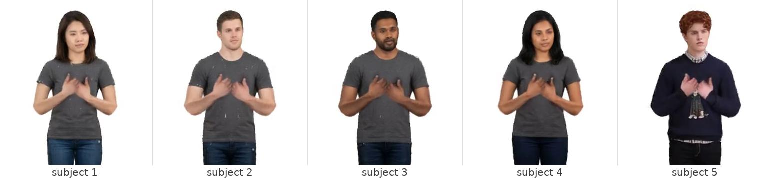
\includegraphics[width=\columnwidth]{fig_identity.pdf}
  \caption{The same generated motion rendered as five subjects, each reconstructed
  from a single photograph with no per-subject optimization, fine-tuning or
  multi-view capture. Body shape is recovered per subject, so proportions differ
  while the motion is identical.}
  \label{fig:identity}
\end{figure}

Fig.~\ref{fig:identity} shows one generated motion rendered as five subjects from
one photograph each. One limitation is visible: in signs where the hands make
contact they render as merged geometry, since Gaussian splatting carries no
surface or collision notion and Gaussians from different hands blend rather than
occlude. As a substantial fraction of signs involve contact, this is a constraint
on Gaussian-splatting sign avatars rather than a tuning issue.

\section{Discussion and Limitations}
\label{sec:discussion}

We can set generated hand articulation to almost any level we like, with a
construction and a paired measurement showing that doing so leaves the sign
untouched. What we cannot do is make the motion be the right sign. Because the
correction provably preserves mean pose and trajectory shape, the flat
correctness column is evidence that these axes are independent, not that our
intervention was harmful. Variance ratios, velocity statistics and the
distributional metrics this literature reports all measure how the hands move,
and can be moved at will without getting closer to the right sign.

One tension deserves stating. \cite{hong2026collapse} report a gloss-level system
satisfying faithfulness at 0.73 while their sentence-level systems fail, reading
this as evidence that paired-data scale is the bottleneck. Ours is also
gloss-level and fails throughout. Our corpus is small and our motion branch is
pretrained on another sign language, but the from-scratch control rules the
second out, leaving data scale as the more plausible explanation and our result
as a constraint on it rather than a refutation.

\noindent\textbf{Limitations.} The released subset covers 124 of WLASL's 2,000
glosses, of which we hold out 25, and correctness is evaluated on one rendered
subject. More importantly, no deaf reader has assessed any output: our metrics
are validated against real signing, the strongest check available to us, but that
is not judgement by a fluent signer. Timing is a persistent weakness, and the
motion branch cannot produce facial articulation at all, which matters because
facial expression carries grammatical function in sign languages.

\bibliographystyle{IEEEbib}
\bibliography{refs}

\end{document}
